\documentclass[../../thesis.tex]{subfiles}
\graphicspath{{\subfix{diagrams/}}}

% \begin{document}
In this section we will look at a number of mertics that are useful for judging the systems performance. In zkSNARK enabled systems, the results must always be considered out of two different point of views. For one, the changes in gas usage are important. After all, this system is built to reduce gas consumption per trade. Another thing to consider, is the performance of the zkSNARK steps that are neccecary to execute and verify\todo{Notarize execution maybe the correct word?}  a circuit. As zkSNARKs rely on complex cryptographic primitives, the generation of proofs can take a long time, even on powerful hardware. We will start by looking at the gas usage results first, and then look at a number of metrics for the zkSNARK circuits. 

\subsection{Gas Cost}
In this system, we have four different operations that require gas to be executed. We will now look at these operations, presenting the measured results. The following three charts are scaled logarithmically on the x-axis. The logarithmical scale was chosen, as these operations have a large overhead (fixed cost) and a porportionally small amount of variable cost. This results in the cost per trade to reduce significalty in the beginning, which can be visualized best on a logarithmic x-axis scale.

\subsubsection{Trade Aggragation}
To break down the gas cost of a trade aggregation batch, we must first differentiate between fixed and variable gas cost that need to be paid per batch and trade. For one, the gas for the net trade, executed on Uniswap, must be paid. This amount varyies, depending on the direction of the net trade, ~142k when trading from Ether and ~167k gas when trading from an ERC20 token. 
 
Another fixed cost to consider is the gas for verifying the zkSNARK proof, along with handling the refund payment of the aggregator and the checks defined in S. \ref{trade_checks}. Executing these costs ~342k gas per aggregation batch. The combined fixed amount of gas per aggregation batch is ~484k/~509k gas, depending on the net trade direction. For each trade in a batch, we must pay 6619 gas, which is used for recreating the data hash, as well as emitting the BalanceUpdate event. When using these numbers, we get the following cost per trade, depending on the batch size. In this diagram, we're using the more expensive net trade (ERC20 to Ether) to calculate the results, which results in the maximum cost per trade for the corresponding batch size. As the difference is small, the difference in gas per trade converges quickly. The theoretical maximum batch size is 1811, which is where Ethereums block gas limit is reached. 

To compare the results to a normal Uniswap trade, we define a break even price, which is equal to the cost of a Uniswap trade. Our system makes sense economically once our gas per trade cost is lower then the break even point. We will use 142k gas as our break even point, which is the best case for a Uniswap trade. The numbers found in this diagram do not contain any gas cost required for making a deposit or withdraw.

\begin{figure}[h]
    \centerline{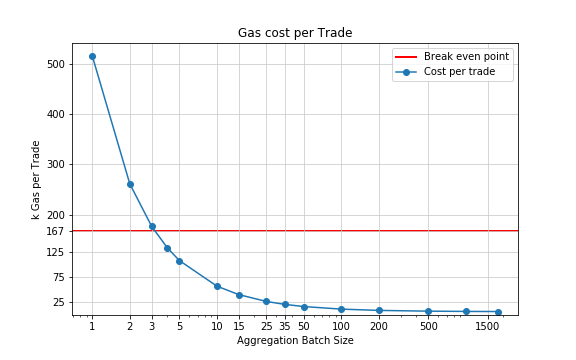
\includegraphics[totalheight=6cm]{diagrams/trade_cost.png}}
    \caption{Gas cost per trade and breakeven point}
    \label{fig:cost_trade}
\end{figure}

\subsubsection{Deposits and Withdraws}
Before a user is able to trade, funds must be deposited into the system. Presenting these results is a bit more diffecult compared to the trade aggregation results for two reasons. For one, the deposits and withdraws are aggregated as one aggregation batch. Since the gas costs for a deposit and withdraw are different, and the number of deposits and withdraws included in a batch is not predicatable, the cost per deposit/withdraw depends on the proportion of deposits and withdraws in a batch. On top of that, the gas cost of an deposit/withdraw also depends on the asset. Ether deposits/withdraws are cheaper than ERC20, which is a result of how tokens are represented on the Ethereum blockchain. For this reason we will present three quartiles for deposits and withdraws, that represent the share of an asset in the batch. For example, as seen in F. \ref{fig:cost_dep}, `25\% Eth' represents the gas cost per deposit if 25\% of deposits in that batch are Ether deposits. While the numbers are a bit inaccurate for smaller batch sizes, it seems like the best approach to present the results overall. 

\paragraph{Deposit Aggregation}
As with the trade aggregation, there is a fixed and a variable gas cost required per batch. For each deposit aggregation we have ~312k gas as a fixed cost. This involves all checks and verifications explained in S. \ref{aggr_deps}. The variable gas cost depends if an Ether or an ERC20 token is deposit. Depositing an ERC20 token requires significantly more gas then sending Ether, as multiple smart-contract interactions are neccecary. An Ether deposit adds ~23k gas, an ERC20 deposit ~116k gas. The maximum batch size is chosen based on the worst-case propotions, in this case only ERC20 deposits and the number of deposits we can include before Ethereum block gas limit is reached. For deposits thats a maximum batch size of 105.

\begin{figure}[h]
    \centerline{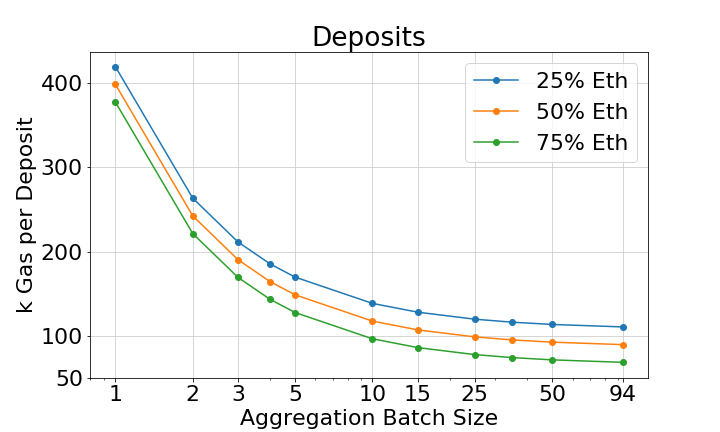
\includegraphics[totalheight=6cm]{diagrams/dep_ET_.png}}
    \caption{Gas cost per deposit assuming different share of Ether deposits}
    \label{fig:cost_dep}
\end{figure}

\paragraph{Withdraw Aggregation}
The fixed costs of the withdraws is equal to the amount specified in the deposit aggregation, as they are being verified in the same batch. As with the deposits, the variable withdraw cost is different, depending if Ether or an ERC20 token is withdrawn. The maximum batch size is chosen based on the worst-case propotions, in this case only ERC20 withdraws and the number of deposits we can include before Ethereum block gas limit is reached. For deposits thats a maximum batch size of 186.

\begin{figure}[h]
    \centerline{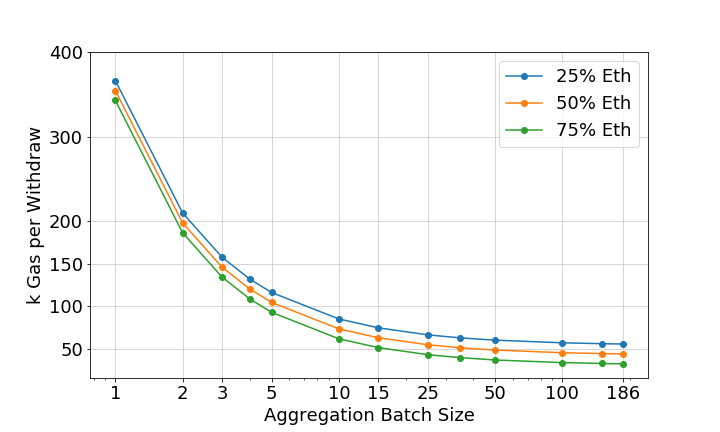
\includegraphics[totalheight=6cm]{diagrams/with_ET_.png}}
    \caption{Gas cost per withdraws assuming different share of Ether withdraws in batch}
    \label{fig:cost_with}
\end{figure}

\paragraph{Combining Deposit and Withdraw Gas Cost}
Modeling the combined gas costs of deposits and withdraws is omitted in the work, as there are to many assumptions that need to be made. As mentioned before, the proportion of Ether and ERC20 operations, as well as the porportion of deposits and withdraws influence the results. For the deposits and withdraws a valid approach was taken to model the potential gas cost, depending on the proportional share of funds. Combining these values, defining the proportional share of deposits and withdraws in an aggregation batch wouldn't yield representetive results, as there are a number of valid combinations that would need to be considered. The diagrams presented above give a clear indication of the potential cost, which suffices for this work.  

\paragraph{Instant Withdraws}
The cost of instant withdraws is also worth considering. Since we're not batching instant withdraws, there is only a fixed cost per withdraw that needs to be paid. Since this hasn't been implemented at the time of writing, a rough estimate of the gas costs can only be provided. To update a balance in a merkle tree with a depth of 16, we need to hash a total of 34 times. 32 times for the merkle inclusion proof and update, twice for hashing the old and new balance. Computing as MiMC hash currently costs ~94k gas, which would bring the cost to around ~3.2m gas per instant withdraw.

\subsection{zkSNARK Circuit Metrics}
Another aspect to consider is the performance of the zkSNARK circuits. The benchmarks for the zkSNARK circuits where performed on a Google Cloud Plattform C2 instance, with 60 vCores (3.1GHz base and 3.8GHz turbo) and 240Gb of memory. This instance was chosen because of the large amount of memory and the fast clock speed. The number of cores doesn’t impact the benchmarking results, as the zkSNARK steps can’t be parallelised at the time of writing.

\subsubsection{Execution Time}
The first obvious metric to consider is execution times of the different steps required to utilize our circuits. 

\paragraph{Compilation and Setup}
Before we can generate any zkSNARK proofs, we have to compile our circuits and run the setup. These two steps only need to be run once per circuit, so they're not significant for the viablilty of this system. However I have the numbers, and it would feel incomplete to not present them. These are the results, for the trade and deposit/withdraw circuit.

\begin{figure}[h]%
    \centering
    \subfloat[]{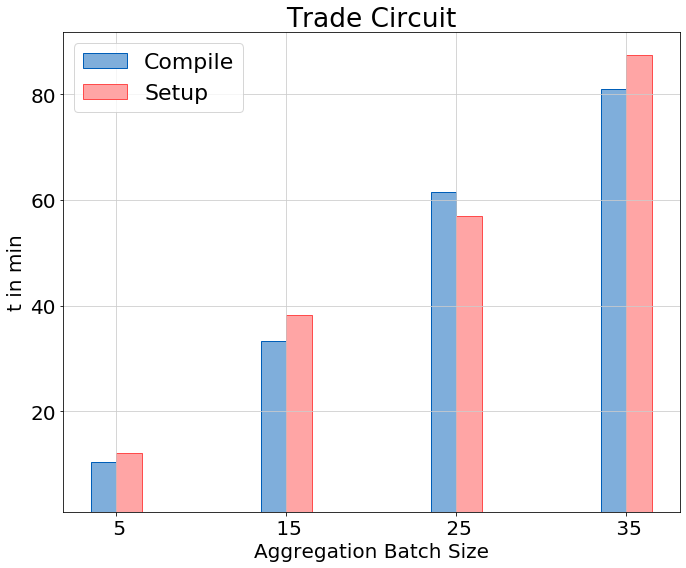
\includegraphics[width=5.9225cm]{diagrams/results_final_trade-compile-setup-time.png} }%
    \qquad
    \subfloat[]{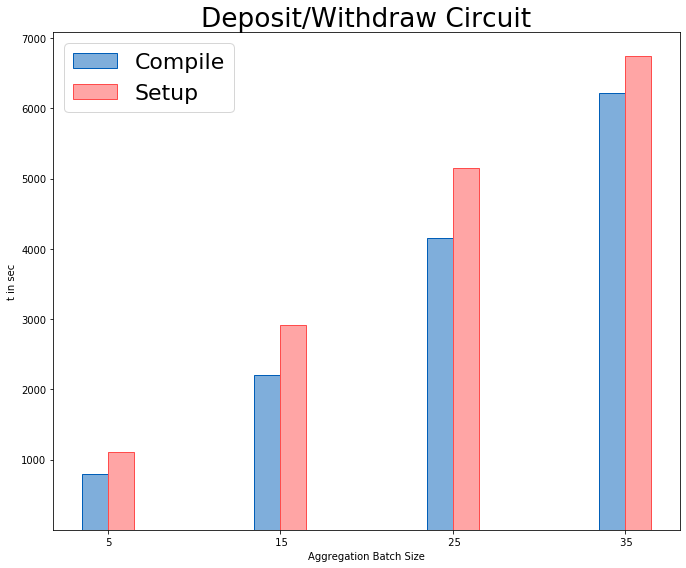
\includegraphics[width=5.9225cm]{diagrams/results_final_dep-compile-setup-time.png} }%
    \caption{Compilation and setup execution times}%
    \label{fig:comp_setup_time}%
\end{figure}

\paragraph{Witness Computations and Proof Generation}
For each aggregation batch we need to first run the witness computation, after which the proof generation can be run. These two steps need to be run for every aggregation batch, so the performance is a indicator for the viability of this system. It decides how long the aggregation of a batch takes, which impacts the pratical application of this system. 

\begin{figure}[h]%
    \centering
    \subfloat[]{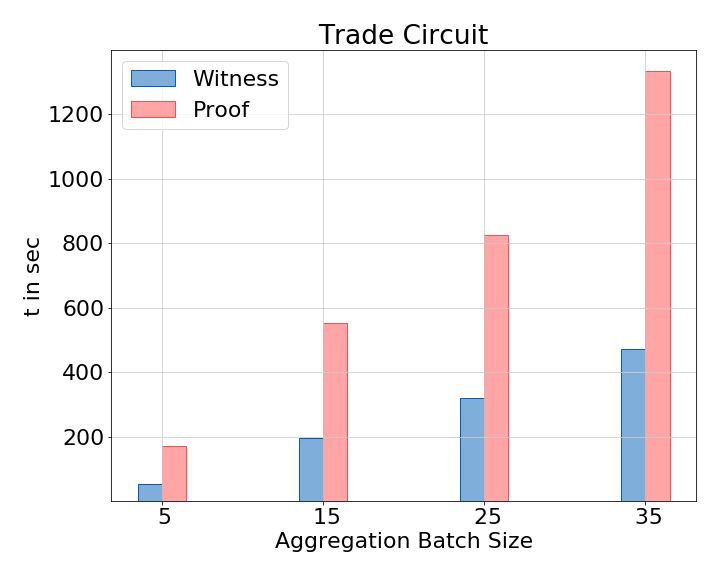
\includegraphics[width=5.9225cm]{diagrams/results_final_trade-witness-proof-time.png} }%
    \qquad
    \subfloat[]{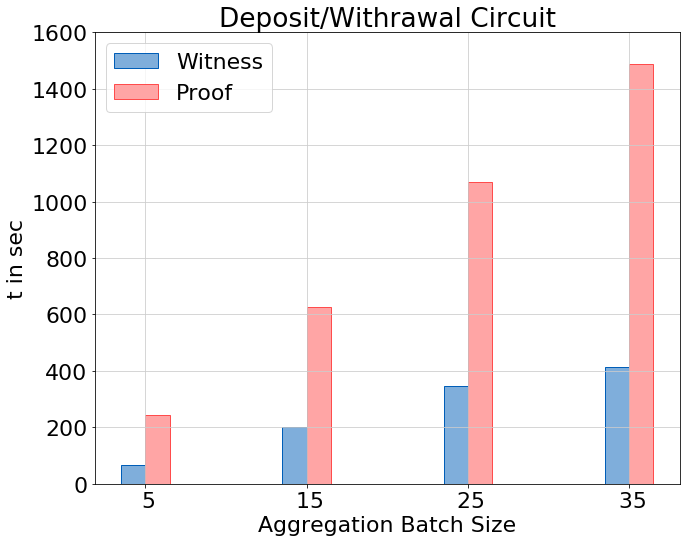
\includegraphics[width=5.9225cm]{diagrams/results_final_dep-witness-proof-time.png} }%
    \caption{Witness computation and proof generation}%
    \label{fig:witness_proof_time}%
\end{figure}

\subsubsection{Memory Usage}
Only looking at the execution times gives us an idea how many operation can be batched. It tells us nothing about the hardware requirements needed for working with circuits of this size. One thing to look at, is the memory used in the different steps. In general, the memory consumption of these processes is high, which is why a server instance with such a large amount of memory was chosen. 

\paragraph{Compilation and Setup}
When measuring the compilation memory consumption, we get a confusing picture. The results don't really make sense, as smaller circuits sometimes require more memory as smaller ones. However, I repeated this measurement on different machines and operating systems, always receiving inconclusive results, similar to these. I watched the compilation on the server with htop, and observed the same amount of memory that the memory usage script was detecting. The script uses the command line tool `ps' to take these measurements, which measures reserved memory by a process. Alternativly, a profiler could be used to measure the actual memory usage. This would impact the performance of the application severly though. As these steps only have to executed once, they are not a meaningful metric. 

\begin{figure}[h]%
    \centering
    \subfloat[]{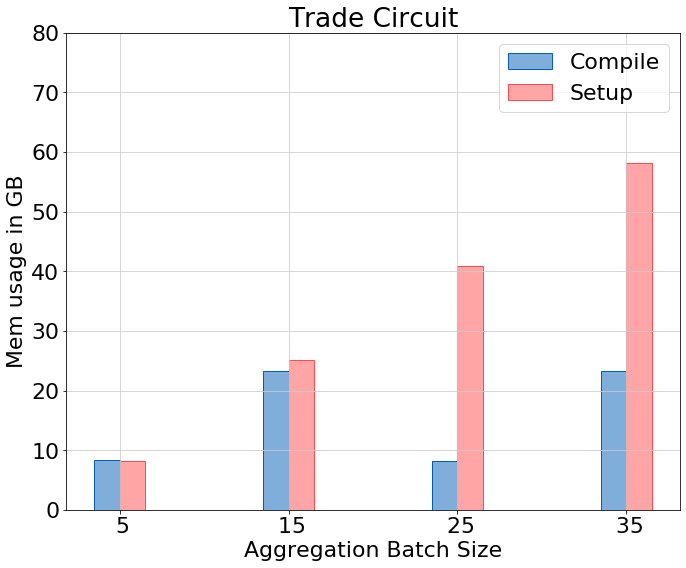
\includegraphics[width=5.9225cm]{diagrams/results_final_trade-compile-setup-mem.png} }%
    \qquad
    \subfloat[]{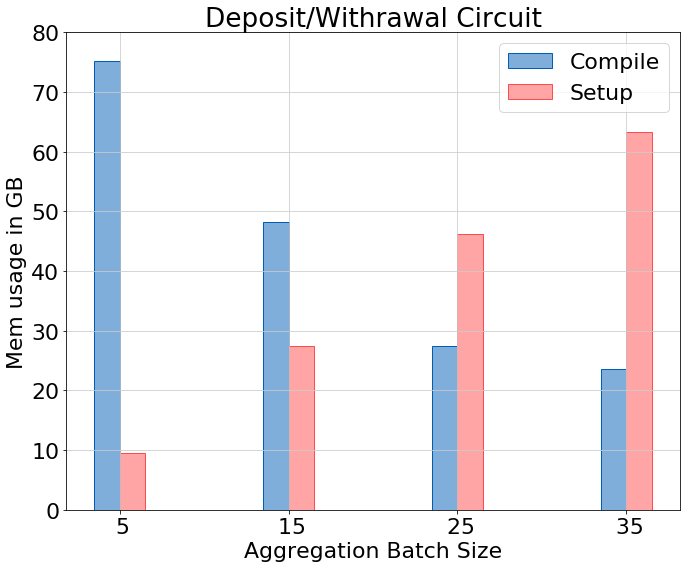
\includegraphics[width=5.9225cm]{diagrams/results_final_dep-compile-setup-mem.png} }%
    \caption{Compilation and setup memory consumption}%
    \label{fig:comp_setup_mem}%
\end{figure}

\paragraph{Witness Computation and Proof Generation}
The memory required for running the witness computation and proof generation is an important metric and dictates the hardware needed for the aggregation process. We need to run these steps for every aggregation batch, so hardware capable of handling the memory requirements must be available.

\begin{figure}[h]%
    \centering
    \subfloat[]{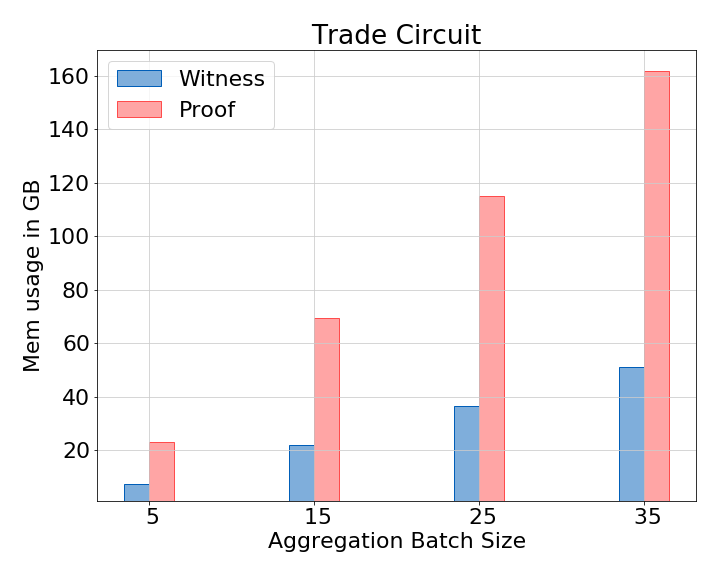
\includegraphics[width=5.9225cm]{diagrams/results_final_trade-witness-proof-mem.png} }%
    \qquad
    \subfloat[]{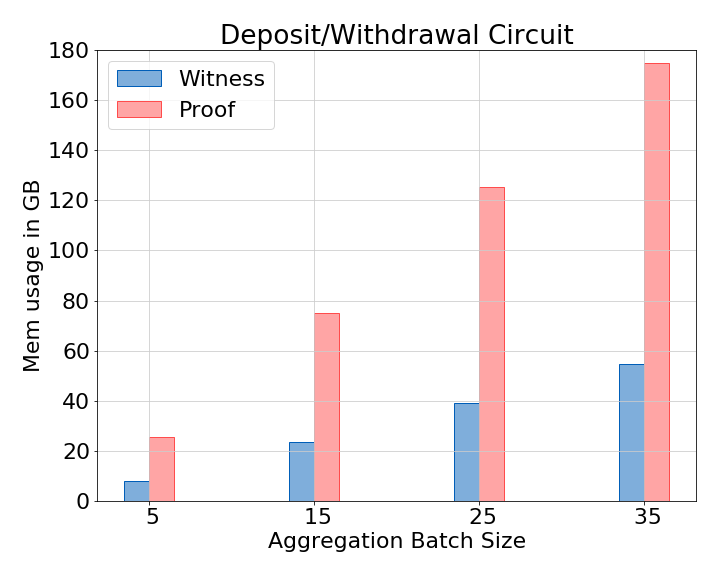
\includegraphics[width=5.9225cm]{diagrams/results_final_dep-witness-proof-mem.png} }%
    \caption{Witness computation and proof generation memory consumption}%
    \label{fig:witness_proof_mem}%
\end{figure}

\subsubsection{Constraints}
Looking at the results, we see that the execution times increase linearly with the batch size. The same pretty much goes for the memory consumption of our circuits. As a general rule, the complexity of a zkSNARK circuit is defined by amount of constraints the circuit is made of. Each additional element in the batch adds a certain number of constraints to the circuit.  Looking at our circuits, we get the following constraint counts for different batch sizes. 

\begin{figure}[h]%
    \centering
    \subfloat[]{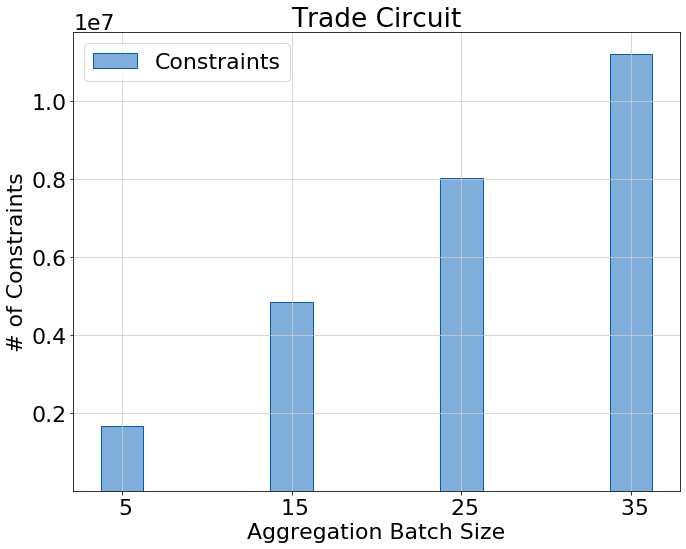
\includegraphics[width=5.9225cm]{diagrams/results_final_trade-constraints.png} }%
    \qquad
    \subfloat[]{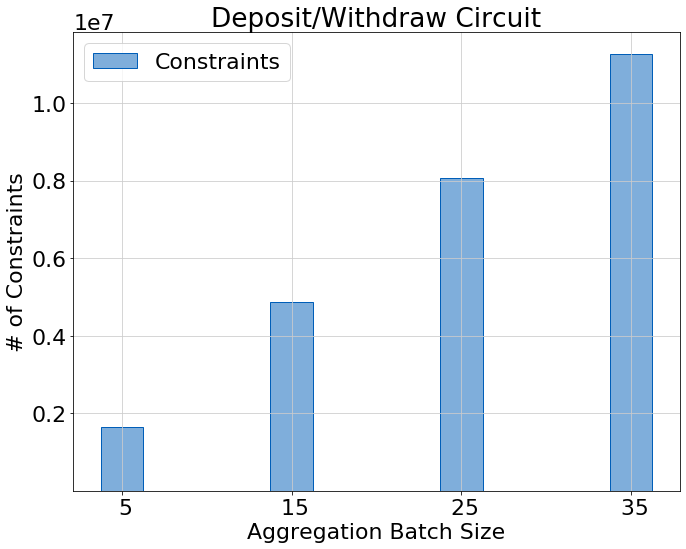
\includegraphics[width=5.9225cm]{diagrams/results_final_dep-constraints.png} }%
    \caption{Constraint count for the circuits in different batch sizes}%
    \label{fig:constraints}%
\end{figure}

\paragraph{Origin of Constraints}
Both circuits can be broken down into three different main segments, that add a certain number of constraints. 1) We need to run the inclusion proof and update the merkle tree. 2) We check the signature and if the balance update follows the signed amounts. 3) We need to compute the data hash. For each of these operations, we get constraint numbers that are added per additional batch element. These numbers where measured by compiling the segments seperatly and checking the constraint count. Comparing these to the total constraint values, we realize that they are higher. This can be explained by the ZoKrates optimizer, which runs a number of optimizations during compilation. As we can see, these values are very similar in both circuits, which is why they have comparable performance.

\begin{table}[h]
    \begin{tabular}{lll}
    \toprule
                                  & Fixed Cost: & Variable Cost:     \\ \hline
    \multicolumn{3}{l}{\textbf{Trade Circuit:}}                      \\ \hline
    \midrule
    Merkle Tree                   & 1          & 179781              \\ \hline
    Verify sig and balance update & 1175       & 25675               \\ \hline
    Data hash                     & 182254     & 184806              \\ \hline
    \multicolumn{3}{l}{\textbf{Deposit/Withdraw Circuit:}}           \\ \hline
    \midrule
    Merkle Tree                   & 1          & 179781              \\ \hline
    Verify sig and balance update & 1          & 28154               \\ \hline
    Data hash                     & 55970      & 184806              \\ \hline
    \bottomrule
    \end{tabular}
\end{table}  \label{constraint_source}
\todo{update constraints for depoist}

\paragraph{Hashing and Constraints} \label{hashing_const}
The MiMC hashing algorithm was used for hashing the merkle tree, as it’s more efficient to use in zkSNARK circuits. The most common hashing operation used in the system is the pair hashing of the merkle tree. Every balance update requires 34 pair hashes in total, 1 for hashing the old balance, 16 for the merkle inclusion proof, 1 for hashing the new balance and 16 for updating the merkle tree. We must also remember, that the pair elements need to be sorted according to their position (left, right), which doubles the constraints in a zkSNARK circuit. On the other hand, we also need to hash the balances in the zkSwap smart-contract for recreating the data hash. In Solidity the sha256 hashing algorithm is a lot cheaper than MiMC. Since we have to recreate the data hash for every batch we want to verify on-chain, the data hash is computed with the SHA256 hashing algorithm. 

\begin{table}[h]
    \begin{tabular}{lll}
    \toprule
    Hashing Op         & Constraints & Gas Usage \\  \hline
    \midrule
    MiMC pair          & 2642        & 38840    \\  \hline
    MiMC pair sorted   & 5285        & 38840    \\  \hline
    SHA256 pair        & 56227       & 2179     \\  \hline
    SHA256 pair sorted & 112453      & 2179     \\  \hline
    \bottomrule
    \end{tabular}
\end{table}

\paragraph{Constraints Processed per Second}
As last metric we want to take a look at, is constraints processed per second in the witness computation and proof generation step. We can calculate these values by dividing the exectution time by the number of constraints. At the time of writing, these steps are not parallelizable and only run on one CPU core. The Loopring protocol claims to have parallelized the libsnark library, which we will look at in S. XX. For this reason we are introducing this metric, as we can compare the outcomes and the potential speed up of parrallelizing. On top of that, this metric can also be helpful to test the performance of the circuits on a CPU with higher clock speed.

\begin{table}[]
    \begin{tabular}{lll}
    \toprule
    batch\_size & Witness: constraints / sec & Proof: constraints / sec \\
    \midrule
    5           & 27604                     & 9685                    \\
    15          & 29615                     & 8417                    \\
    25          & 29088                     & 9612                    \\
    35          & 27797                     & 8382                    \\
    \midrule
    Average     & 28526                     & 9024                    \\
    \bottomrule 
    \end{tabular}
\end{table}\label{const_per_sec}

\paragraph{Constraints per GB Memory}